\section{Design}
\label{design}

\subsection{AI Selection Criteria}
\label{subsection:criteria}
Performing an epic breakdown involves a combination of clustering related requirements, specifications, and details along with the further breakdown of complex info into smaller stories and tasks. Clustering can be performed in either supervised or unsupervised learning. Supervised learning requires the existence of a data set that has been correctly labeled. Although the team might be able to generate general data set of decomposed epics, we concluded that an typical epic might have too many subjects, and we would not be able to produce any accurately labeled model for training purposes. 

Additionally, for the stated purpose of increasing consistencies, we made the assumption that the decomposition process would not rely upon historical project information, such as previously completed epics or sprints. As a result, unsupervised clustering techniques were chosen as it couldo be equally applicable to new and old projects alike.

The last criteria for the text processing approaches was that we would not attempt to generate ``new'' information based on given input. This was due to the previously discussed lack of data, specific to the project domain, that could be used to potentially generate stories and tasks. Table \ref{table:ai} summarizes the decisions we made regarding the selection of AI techniques.

\begin{table*}[h]
	\caption{AI design choices}
	\label{table:ai}
	\begin{tabularx}{\textwidth}{|p{3cm}|p{3cm}|p{2cm}|X|}
	\hline
	Component & Options & Choice & Reasoning\\
	\hline
	Epic Decomposition & 
	\begin{minipage}{0.15\textwidth}
		\begin{itemize}
		\item KMeans
		\item Meanshift
		\item DBSCAN
		\item OPTICS
		\end{itemize}
	\end{minipage} &
	Mean-shift & All of the mentioned clustering algorithms are dynamic as they do not require the number of clusters as input. Mean-shift only requires the size of the region to search through (bandwidth), which can be estimated, where all other options require arbitrary values to create clusters.\\
	\hline
	Story Optimization & 
	\begin{minipage}{0.15\textwidth}
		\begin{itemize}
		\item TF-IDF
		\item SIF
		\item Word2vec
		\item Cosine simularity
		\item Word mover's distance
		\end{itemize}
	\end{minipage} &
	\begin{flushleft}
	SIF with word2vec and Cosine similarity
	\end{flushleft} & TF-IDF is the most simple for word embedding. SIF with word2vec can achieve a higher accuracy than TF-IDF with the custom word2vec model that is relevant to the topic. WMD is far more expensive to calculate, especially on longer texts. Cosine similarity can give the same performance without losing too much semantic similarity.\\
	\hline	
	Task Generation & 	
	\begin{minipage}{0.15\textwidth}
		\begin{itemize}
		\item Sentence classification
		\end{itemize}
	\end{minipage} & Sentence classification & There is a need to split up the different types of sentences, such as complex and compound, into simple sentences, in order for them to be manipulated into tasks. To do this, sentence classification is the necessary first step.\\
	\hline	
	\end{tabularx}
\end{table*}

\subsection{Epic Decomposition}
Through manual decompositions of epics into stories it was identified that the process fundamentally involved the categorization of requirements and specifications. From such, text clustering techniques based upon the vectorization of the contents of epics. Each requirement, assumed to be in the form of a complete sentence or distinguishable section, is vectorized and normalized so a comparison can be performed.

Based on a series of tests on a simpler text clustering problem, K-means, a non-deterministic centroid-based clustering technique, yielded the best results when it came to creating consistent clusters of requirements. The downside to K-means is that it requires the number of clusters to be identified, forcing there to be user input or an estimation to be made. Since it was a goal to have the app be applicable to a large range of epics, in terms of topic and size, issues such as DBSCAN, OPTICS, and Mean shift were explored as they are dynamic and do not require the number of clusters to be specified. DBSCAN/OPTICS are density-based clustering techniques and Mean shift is a centroid-based clustering technique. Ultimately, it was decided to go with Mean shift since the implementation of the technique included an estimation of the cluster sizes, thus requiring no external input.

\subsection{Story Optimization}
Story optimization is further breaking down a story to if it contains more than one story or software feature that needed to be achieved. For story optimization, sentence similarity is high priority. 

A pre-trained Word2Vec model was used to extract the features out of sentences. A sentence embedding technique called SIF embeddings (Smooth Inverse Frequency) was used to compute sentence embeddings as a weighted average of word vectors. Using the features, a comparison was made by calculating the cosine similarity between sentences. 

The result was the similarity coefficient between sentences and it could be used to group sentences together based on their degree of similarity. A function decision was implemented to correctly group sentences from the similarity coefficient using a specified threshold level. 

\subsection{Task Generation}

Task generation was identified as the process of breaking down a requirement into its most simplest form. Based on the criteria laid out in Section \ref{subsection:criteria}, simplification on the existing input of requirements could be completed by deconstructing complex sentences into simple sentences. 

The first process to break down sentences was to use parts-of-speech tagging to remove any unnecessary words from the sentence; this was done by identifying stopwords, since simple sentences contain only one subject and predicate. Therefore, using the word dependency we were able to determine which words were connected to the subject. By making sure the sentence contained one subject and verb we were able to create a complete simple sentence. Everytime a new subject was found that meant a new sentence was needed. Each simple sentence generated from the stories can then be suggested as tasks.

\subsection{Process Flow}

\begin{figure*}
\centerline{\includegraphics[width=\textwidth,height=\textheight,keepaspectratio]{./figure/ExampleDataFlowDiagram.png}}
\caption{Simplified Data Flow diagram outlining the flow of the decomposition processes}
\label{fig:ExampleDataFlowDiagram}
\end{figure*}\

There is an overall linear flow, as seen in Figure \ref{fig:ExampleDataFlowDiagram} to AI4Agile’s main processing: Epic Decomposition, Story Optimization, and then Task Generation. Additionally, the relationship graph may be generated at any point and is independent of the previously mentioned flow. It is possible that the starting point in the flow may vary between uses. For example, a user may have manually entered in all their overarching user stories for their epic, forgoing the use of the Epic Decomposition process. From these entered stories, either story optimization or task generation may be performed.

\begin{figure*}
\centerline{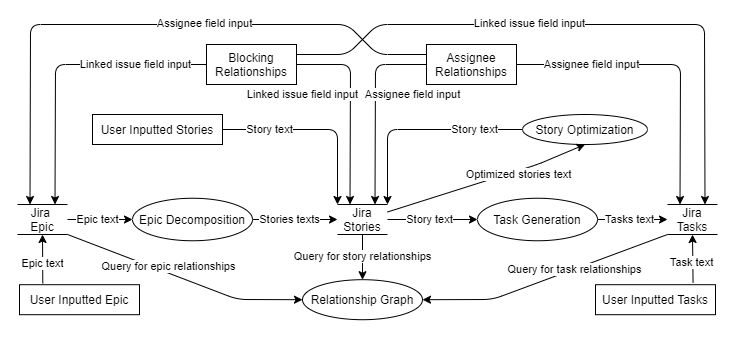
\includegraphics[width=\textwidth,height=\textheight,keepaspectratio]{./figure/DataflowDiagram.png}}
\caption{Data Flow diagram showing the various entry points, sources of data, and processes within Jira and AI4Agile}
\label{fig:DataFlowDiagram}
\end{figure*}
Placeholder cause I need to reference Figure \ref{fig:DataFlowDiagram}
\subsection{Relationship visualization}
The purpose of the relationship graph is to give users a visual representation of the dependencies between a selected issue in Jira and the issues that are related to it. Currently in Jira, hierarchies are shown minimally in such ways as dropdown lists from epics, or lists within an issue selection pane of either children or explicitly specified blocking/cloning/similarity relationships. This graph provides a way to view those relationships in one place at a glance, for ease of visual understanding.
\subsection{User Interface and Experience}
For the user interface and experience, a combination of prototyping and stakeholder meetings went into the decisions displayed in Table \ref{tab:UIUXDesignChoices}. The highest priority was to make the interface as intuitive and easy to use as possible, to fall in line with the larger project goal of saving users time throughout the agile development process.
\begin{table*}[h]
	\caption{UI and UX Design Choices}
	\begin{tabularx}{\textwidth}{|p{3cm}|p{3cm}|X|}
	\hline
	Options & Choice & Reasoning\\
	\hline
	\begin{itemize}
		\item Suggestion Format
		\item Chatbot
	\end{itemize} &
	Suggestion format & A conversation element can slow down the process and ease of use. A suggestion format was chosen to avoid the case where using the plugin as one who is familiar with the project and decomposition methods would slow down a decomposition process instead of accelerating it.\\
	\hline
	\begin{itemize}
		\item Templated epic input
		\item Unrestricted epic input
		\item Semi-structured epic input via guidelines
	\end{itemize} &
	Semi-structured epic input via guidelines & A template was deemed too restrictive and time consuming for the user, but unrestricted input was infeasible for AI processing. Thus, the choice was to present the user with guidelines in the user manual for what the optimal structure of an epic would be for use with this plugin.\\
	\hline	
	\begin{itemize}
		\item External database use
		\item Strictly Jira database use
	\end{itemize} & 
	Strictly Jira database use & There is a need to split up the different types of sentences, such as complex and compound, into simple sentences, in order for them to be manipulated into tasks. To do this, sentence classification is the necessary first step.\\
	\hline
	\begin{itemize}
		\item Relationship Graph as tree
		\item Relationship graph as clusters
		\item Relationship graph as tree and clusters
	\end{itemize} & 
	Relationship graph as tree and clusters & While the original concept had the relationships as clusters, it was determined from stakeholder input that a tree format would likely be more intuitive to the user base. At the same time, if the relationships to be shown are only developer assignments, the lack of parent-child relationships suggested clustering was still the sensible choice.\\
	\hline
	\begin{itemize}
		\item Undo functionality for story/task creation
		\item Preview button for story/task creation
		\item Iterative creation process
	\end{itemize} & 
	Iterative creation process & With undo functionality, there were issues such as where it would make sense to have such a thing, how far after the action it should be able to be undone, and how much additional effort would be needed to implement it. The reasoning behind this feature in general was for new users to be able to experiment with the plugin without fear of consequences. It was determined that switching to an iterative process, where users can create one story or task at a time from the suggestions, would serve this same purpose to lessen potential consequences and still allow users to experiment. As a result of the iterative creation process, the need for a preview system was eliminated.\\
	\hline
	\end{tabularx}
\label{tab:UIUXDesignChoices}
\end{table*}